Being acquainted with the premise, we now possess a coarse understanding of the relevant mathematical scaffold required to understand dimensionality reduction.
Additionally, we became aware of the potential pitfalls that hold true to the subject in general.
Therefore, we are now ready to take a closer look on how to categorise and associate various techniques.

\subsubsection{Linear vs. non-linear problems}
The utmost category, used to differentiate between various techniques is fortunately mutually exclusive to any method.
Thanks to this characteristic, we can distinctively classify and associate a given technique.
This allocation, contrary to the following classifications, is the one that considers the domain of the problem.
Thus, it requires special attention by its users since it can easily be used erroneously.
We need to understand the gross patterns in the data set we need to operate on.

The below figure \ref{fig:linearvsnonlinearproblems} illustrates and contrasts the general patterns that we need to identify.\vspace*{4mm}

\renewcommand{\tikzscale}{1.25}
\begin{figure}[h]
	\begin{subfigure}{0.48\textwidth}
	    \caption{Linear problems}
		\begin{tikzpicture}[scale=\tikzscale]
	% AXIS
	\draw[->,ultra thick] 
		(0,0)--(5,0) 
			node[midway, below,yshift=-1mm]{$x_1$};

	\draw[->,ultra thick] 
		(0,0)--(0,5) 
			node[midway, left, xshift=-1mm]{$x_2$};

	% DIAGONAL LINE
	\draw[-, dashed] 
		(0.2,0.2)--(4.5,4.5)
				;

	% NODES

	\begin{scope}[color=iwiPurple,line width=1.25pt]
	 	\newcommand{\lowerarray}{%
	 		{2.3,1.7},{3.3,0.7},{1.2,0.5},{2.7,1.2},{2.4,1.4},{1.8,1.2},{3.4,2.4},{3.2,0.5},{1.3,0.7},{1.2,0.7},{3.7,1.8},{3.5,0.6},{2.4,0.6},{3.3,2},{1.5,0.9},{1.3,0.8},{1.3,0.7},{3.6,0.6},{3.2,2},{3.8,1.7},{1,0.5},{2.8,0.6},{3.9,2.5},{2.6,0.9},{3.7,1.7},{2.3,0.6},{3.9,1.4},{3.8,2.5},{1.4,0.7},{1.7,0.9},{3,2.4},{1.9,0.8},{2,1.5},{2.4,1.6},{1.4,0.9},{1.9,0.9},{2.8,1.7},{1.6,0.5},{3.9,0.8},{3.9,1.8},{2.3,0.7},{2.5,1.6},{1.4,0.7},{4,3.5},{3.1,0.9},{3.4,2.5},{3.3,2.2},{4,1.5},{2,1.5}%
	 	}

		\foreach \i in \lowerarray {
		 	\draw (\i) 
		 		circle (2pt);
		}
 	\end{scope}

	\begin{scope}[color=hkaRed,line width=1pt]
	 	\newcommand{\upperarray}{%
	 		{2.9,4},{1.7,2.7},{3.2,3.8},{2.6,3.8},{2.5,3},{3.5,4.5},{2.3,4.2},{2.8,4.3},{2.5,4.2},{4,4.5},{3.6,4.2},{3.8,4.5},{4,4.5},{1.4,4.1},{3.6,4.1},{1.2,3.7},{3.7,4.2},{3.5,4.4},{1.7,4.1},{2.3,4},{2.2,2.7},{1.4,4.2},{2.3,3.7},{4,4.5},{2.6,3.8},{1.9,2.4},{3.3,4.3},{2.8,4.4},{1.8,2.8},{1,3.1},{2.1,4.4},{1.2,3.7},{4,4.5},{2.2,3.5},{3.5,4.3},{1,1.5},{1.2,3.1},{2.2,2.9},{1.8,2.3},{1.4,4.1},{3.7,4.3},{3,3.9},{3.4,4},{1.8,3.7},{1.8,4.3},{2.5,4},{3.7,4.4},{2.8,3.8},{1.5,4.1}%
	 	}

		\foreach \i in \upperarray {
		 	\node[isosceles triangle,draw,isosceles triangle apex angle=60,rotate=90, minimum size=3pt,inner sep=0pt] (T) at (\i){};
		}

	 \end{scope}

\end{tikzpicture}

	    \label{subfig:linearproblems}
	\end{subfigure}
	\hfill
	\begin{subfigure}{0.48\textwidth}
	    \caption{Non-linear problems}
		\begin{tikzpicture}[scale=\tikzscale]
	% AXIS
	\draw[->,ultra thick] 
		(0,0)--(5,0) 
			node[midway, below, yshift=-1mm]{$x_1$};

	\draw[->,ultra thick] 
		(0,0)--(0,5) 
			node[midway, left, xshift=-1mm]{$x_2$};

	% DELIMITER CIRCLE
 	\draw (2.5,2.5)[dashed]
 		circle (42pt);

	% NODES

	\begin{scope}[color=iwiPurple,line width=1.25pt]
	 	\newcommand{\innerarray}{%
	 		{2.4,2.5},{1.8,1.8},{3,3.4},{3.4,2.1},{1.9,2.8},{1.6,2.1},{2,1.6},{2.7,2.7},{3,3.5},{3,2.4},{2.6,1.5},{2,2.6},{2.7,3},{1.5,3},{2.6,2.7},{3.1,2},{1.9,3.4},{2,2.6},{3,2.2},{1.6,3.2},{2.8,1.5},{2.3,2.7},{2.6,2.5},{2.5,3.5},{3.3,1.7},{2.1,1.8},{2.2,2.1},{1.6,2.8},{3.1,2.9},{1.7,2.2},{1.6,2.9},{2.7,2.7},{2,1.8},{3,1.7},{3.4,2.7},{3.4,2.3},{2.1,2.6},{1.7,1.7},{2.9,3.2},{1.6,3},{3,2.9},{2.4,2.6},{2.5,2.8},{3.3,3.2},{2.9,2.2},{2.3,2.2},{2.8,2.7},{2,2.5},{3.1,1.8}%
	 	}

		\foreach \i in \innerarray {
		 	\draw (\i) 
		 		circle (2pt);
		}
 	\end{scope}

	\begin{scope}[color=hkaRed,line width=1pt]
	 	\newcommand{\outerarray}{%
	 		{0.2,0.6},{0.9,0.9},{1.3,0.4},{0.4,0.5},{0.7,1.1},{1.2,0.2},{1.3,0.4},{0.3,0.4},{0.5,1.4},{0.9,1.2},{0.5,0.4},{0.3,0.3},{4.3,4.3},{4.5,4.1},{4.2,4.5},{3.9,4.4},{3.7,4.5},{3.9,3.7},{4.4,4.1},{4.2,4.4},{3.9,3.7},{3.9,4},{3.8,3.6},{4,4},{4.4,0.6},{4.1,1.4},{3.7,1.1},{3.9,0.6},{4.3,0.3},{4.2,1.4},{4.2,0.7},{3.8,1.3},{4.1,0.7},{4.1,1.1},{4.3,1.2},{4.3,1.4},{0.2,4.5},{1.1,4.3},{1.2,4.5},{0.8,3.6},{0.8,3.6},{0.4,4.2},{0.5,4.2},{0.8,3.7},{0.2,3.5},{0.4,4.3},{0.9,3.8},{0.5,4.5},{3.2,0.8},{3.5,0.8},{3.3,0.8},{2.7,0.8},{2.1,0.5},{2.3,0.6},{2,0.6},{3.4,0.8},{3.1,0.5},{2.7,0.8},{3.5,0.7},{2.6,0.5},{0.8,3.1},{0.7,2.4},{0.7,3.1},{0.8,2.6},{0.6,2.1},{0.5,2.9},{0.8,2.2},{0.7,2.9},{0.8,2.4},{0.7,3.1},{0.8,3.4},{0.7,2.2},{3.4,4.4},{2.8,4.2},{2.4,4.5},{3.5,4.5},{3.4,4.2},{3.1,4.5},{2.9,4.3},{2.5,4.5},{3.4,4.5},{2.2,4.2},{3.1,4.5},{2.7,4.5},{4.5,3},{4.5,2.7},{4.3,2.3},{4.2,2.3},{4.2,2.9},{4.5,2.5},{4.2,2.6},{4.4,2.1},{4.2,2.1},{4.2,2},{4.3,3.4},{4.4,2.2}%
	 	}

		\foreach \i in \outerarray {
		 	\node[isosceles triangle,draw,isosceles triangle apex angle=60,rotate=90, minimum size=3pt,inner sep=0pt] (T) at (\i){};
		}

	 \end{scope}

\end{tikzpicture}

	    \label{subfig:nonlinearproblems}
	\end{subfigure}
\caption{Linear vs. non-linear problems.}
\label{fig:linearvsnonlinearproblems}
\end{figure}

As we can see in figure \ref{subfig:linearproblems}, a linear problem is given when we are able to identify a straight line, or any \gls{hyperplane}, to split the data into unambiguous subsets.
Intuitively and, as we will later examine, factually, these types of problem are comparably easy to solve.

A non-linear problem, as pictured in figure \ref{subfig:nonlinearproblems}, already looks more complex on the first glance.
And indeed, we will illuminate the solution approaches to this scenario and elaborate on its comportment.

\clearpage

\subsubsection{Projection vs. manifold learning}
% taken from ch 8 in géron's book

In this section, we will compare the general solution approaches available which can be utilised to solve both linear as well as non-linear problems. \cite{HandsOnMLCh8}

\todo{Not quite true, revisit this. \cite{Lee2007NonlinearDR} cite this.}

\renewcommand{\tikzscale}{0.33}
\begin{wrapfigure}[13]{r}{0.62\textwidth}
	\vspace*{-8mm}
	\centering
	\newcommand{\textproperties}[1]{\textcolor{gray}{\textbf{#1}}}
\newcommand{\circlecolor}{hkaRed}
\newcommand{\circlesize}{6}


%%%%%%%%%%%%%%%%%%%

\begin{tikzpicture}[scale=\tikzscale]
 	\node at (12.5,7) {\textproperties{example data set in 2D space:}};
	% AXIS
	\draw[->,ultra thick] 
		(0,0)--(25,0) 
			node[midway, below, yshift=-1mm]{$x$};

	\draw[->,ultra thick] 
		(0,0)--(0,5) 
			node[midway, left, xshift=-1mm]{$y$};

	% NODES

	\begin{scope}[color=\circlecolor]
	 	\newcommand{\datapoints}{%
	 		{24,1},	{23,1},	{21,3},	{4,2},	{8,1},	{20,2},	{19,1},	{17,2},	{7,2},	{24,1},	{5,2},	{2,3},	{5,2},	{9,1},	{24,1},	{14,2},	{12,2},	{12,1},	{17,1},	{24,2},	{12,2},	{18,2},	{18,1},	{12,1},	{10,3},	{24,2},	{24,3},	{22,1},	{9,2},	{16,2}%
	 	}

		\foreach \i in \datapoints {
		 	\filldraw (\i) 
		 		circle (\circlesize pt);
		}
 	\end{scope}

%%%%%%%%%%%%%%%%%%%

	\draw[->,ultra thick] (0,-6)--(25,-6);
 	\node at (12.5,-4) {\textproperties{projection on x \gls{hyperplane}:}};
	\node at (1,-7) {$x$};

	\begin{scope}[color=\circlecolor]
	 	\newcommand{\datapoints}{%
	 		{24,-6},	{23,-6},	{21,-6},	{4,-6},	{8,-6},	{20,-6},	{19,-6},	{17,-6},	{7,-6},	{24,-6},	{5,-6},	{2,-6},	{5,-6},	{9,-6},	{24,-6},	{14,-6},	{12,-6},	{12,-6},	{17,-6},	{24,-6},	{12,-6},	{18,-6},	{18,-6},	{12,-6},	{10,-6},	{24,-6},	{24,-6},	{22,-6},	{9,-6},	{16,-6}%
	 	}

		\foreach \i in \datapoints {
		 	\filldraw (\i) 
		 		circle (\circlesize pt);
		}
 	\end{scope}

%%%%%%%%%%%%%%%%%%%

 	\node at (12.5,-10) {\textproperties{projection on y \gls{hyperplane}:}};
	\draw[->,ultra thick] (0,-12)--(25,-12);
	\node at (1,-13) {$y$};

	\begin{scope}[color=\circlecolor]
	 	\newcommand{\datapoints}{%
	 		{6,-12},	{6,-12},	{18,-12},	{12,-12},	{6,-12},	{12,-12},	{6,-12},	{12,-12},	{12,-12},	{6,-12},	{12,-12},	{18,-12},	{12,-12},	{6,-12},	{6,-12},	{12,-12},	{12,-12},	{6,-12},	{6,-12},	{12,-12},	{12,-12},	{12,-12},	{6,-12},	{6,-12},	{18,-12},	{12,-12},	{18,-12},	{6,-12},	{12,-12},	{12,-12}%
	 	}

		\foreach \i in \datapoints {
		 	\filldraw (\i) 
		 		circle (\circlesize pt);
		}
 	\end{scope}


\end{tikzpicture}

	\captionsetup{justification=centering}
	\caption{Simple example of a projection}
    \label{fig:projectionExample}
\end{wrapfigure}

\paragraph{Projection} In contrast, this is the trivial concept of the two. The idea is to project the data points onto a \gls{hyperplane} which summarises the data with as little information loss as possible.

Figure \ref{fig:projectionExample} illustrates this in a simple example.
As we can observe, when we pick the right \gls{hyperplane}, such as the x axis in the example, we lose far fewer information than if we would have picked the y axis.


\paragraph{Manifold learning} This concept is significantly more difficult to get a hold of.
Significant breakthroughs \cite{ma2012manifold} in this field were accomplished in the year 2000 in the significant and commonly cited paper \emph{A global geometric framework for nonlinear dimensionality reduction}. \cite{tenenbaum2000global}
To understand the basic idea, we will demonstrate its behaviour to get an idea of the problem using the popular swiss roll data set pictured in figure \ref{fig:swissrollfull}.


\noindent
\begin{minipage}[c]{0.4\linewidth}
%
\vspace*{6mm}
\begin{center}
	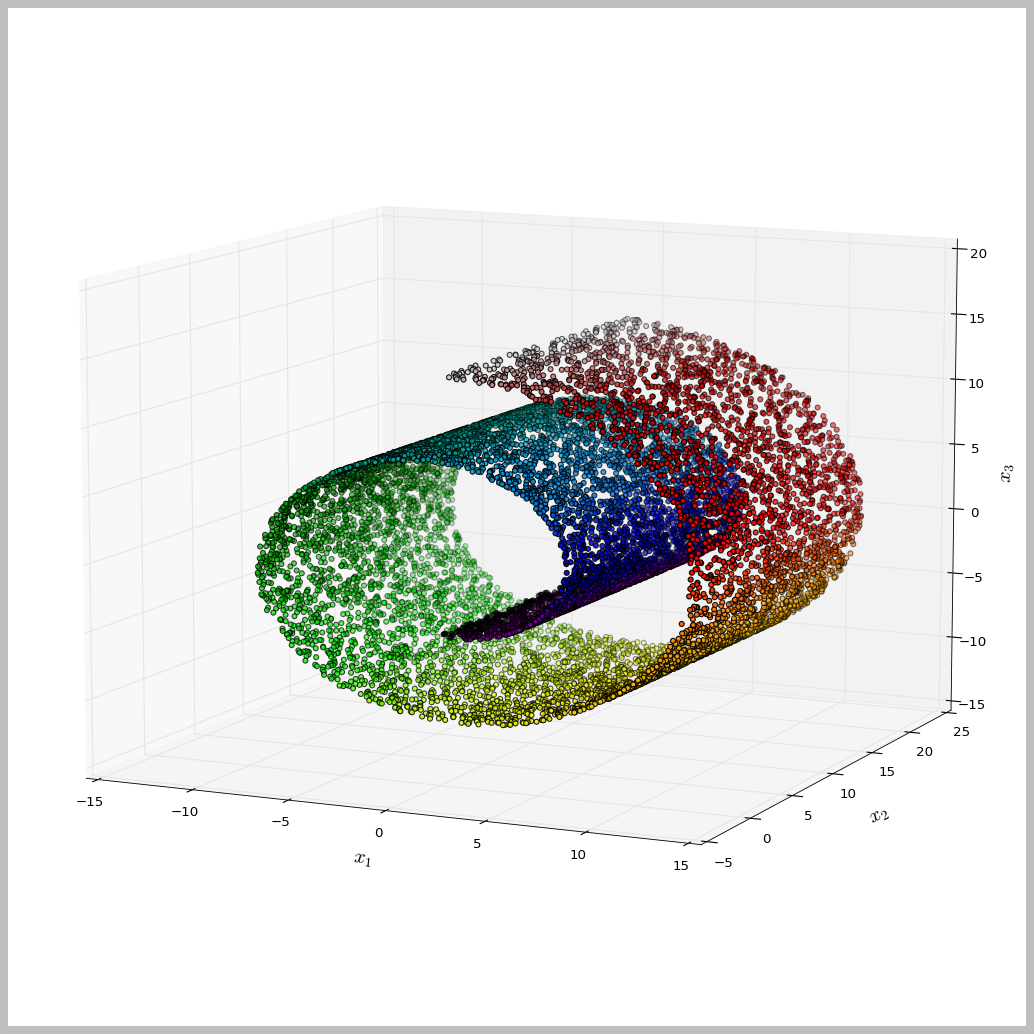
\includegraphics[width=0.9\textwidth]{external_content/graphs/swiss_roll.png}
	\captionsetup{justification=centering,type=htypei}
	\captionof{figure}{Swiss Roll generated from scikit-learn \cite{scikit-learn}}
	\label{fig:swissrollfull}
\end{center}
%
\end{minipage}\hfill%
\begin{minipage}[c]{0.55\linewidth}
Before demystifying this problem, we will then dive into various methods how to bend and twist high-dimensional data into lower-dimensional spaces.

Our goal is to avoid confusing projections such as shown in figure \ref{fig:swissrollprojection}:

\begin{center}
	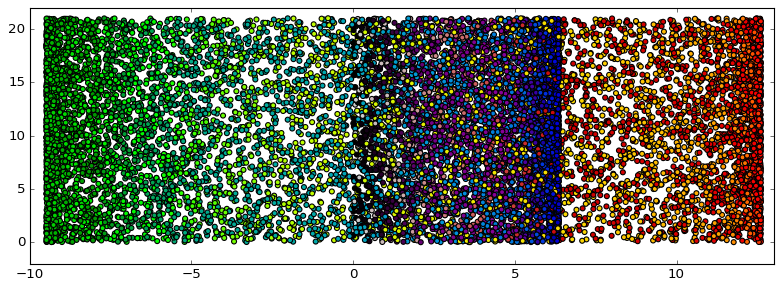
\includegraphics[width=0.8\textwidth]{external_content/graphs/swiss_roll-projection.png}
	\captionsetup{justification=centering,type=htypei}
	\captionof{figure}{Representation in 2D\\ of a projected swiss role}
	\label{fig:swissrollprojection}
\end{center}
\end{minipage}%

\clearpage


%%%%%%%%%%%%%%%%%%%%%%%%%%%%%%%%%%%%%%%%%%%%%%%%%%%%%%%%%%%%%%%%


\subsection{Principal Component Analysis (PCA)}

\begin{itemize}
	\item First approaches made in 1901 using simple projections. \cite{pearson1901liii}
	\item Primarily used for feature extraction \cite{PythonMachineLearningCh5}
	\item Unsupervised method \cite{PythonMachineLearningCh5}
	\item Is an eigenvector problem \cite{MultilinearSubspaceLearningCh2}
	\item scikit-learn implemented this version \cite{minka2000automatic} to guess the output dimesionality. \cite{halko2009finding} is used to decompose the input matrix.
	\item \gls{pca} assumes that the data is centered around the origin \cite{HandsOnMLCh8}. scikit-learn takes care of that.
	\item \gls{svd} is a matrix factorization technique \cite{HandsOnMLCh8}
\end{itemize}


\clearpage

\paragraph{full \gls{svd}} \label{svd}

According to \cite{wright2001large}

$$\bigo{N^3}$$

\clearpage

\paragraph{\gls{arpack}}

According to \cite{wright2001large}

$$\bigo{N^2}$$

\clearpage

\paragraph{randomised}

According to this \cite{HandsOnMLCh8}

$$\bigo{d^3}$$


\clearpage

\paragraph{Conclusion}

\clearpage


%%%%%%%%%%%%%%%%%%%%%%%%%%%%%%%%%%%%%%%%%%%%%%%%%%%%%%%%%%%%%%%%


\subsection{Non-Linear Example}
\begin{itemize}
	\item First introduced by \cite{scholkopf1998nonlinear}
	\item According to this ...%\cite{}
\end{itemize}

$$\bigo{TBA}$$

\clearpage

\begin{center}
	\textit{Not sure what comes here, but most certainly going to be two pages}
\end{center}

\clearpage

